% !TeX root = ../../../main.tex

Deep-inelastic structure functions can be evaluated with several public codes
such as \apfel~\cite{Bertone:2013vaa} and \textsc{\small
QCDNUM}~\cite{Botje:2010ay}.
%
These various available DIS codes differ in the accuracy with which structure
functions can be computed, whether they are based on the $x$-space or the
$N$-space formalism, the treatment of heavy quark mass effects and of target
mass corrections, the availability of polarised and time-like coefficient
functions, and the inclusion of QED corrections among  other considerations.

\yadism is a new actor on this scene, being created as a framework for the
evaluation of DIS structure functions from the same family as the
\textsc{\small EKO}~\cite{Candido:2022tld} DGLAP evolution code (cf.\
\cref{ch:eko}).
%
The open source \yadism code can be obtained from its GitHub repository
\begin{center}
  \ghurl{NNPDF/yadism}
\end{center}  
together with a detailed documentation, tutorials, and user-friendly examples
\begin{center}
  \url{https://yadism.readthedocs.io/}
\end{center}  
One of the main advantages of \yadism is that it is integrated with the fast
interpolation grid toolbox \pineappl~\cite{Carrazza:2020gss},
and hence DIS structure functions can be treated on the same footing as
hadronic observables from the point of view of \pdf{} fitting and related
applications.
%
\pineappl provides a unique grid format, with application programming
interfaces (APIs) for different programming languages and a user-friendly
command-line interface to manage the grid files (cf.\ \cref{ch:pine}).
%
Furthermore, \yadism implements the available N$^3$LO DIS coefficient
functions, which combined with (approximate)  N$^3$LO evolution and heavy quark
matching conditions available in \eko provide theoretical
calculations required to carry out a N$^3$LO \pdf{} determination.
%
\yadism will be described in detail in an upcoming publication~\cite{yadism},
and here we summarise its main features, in particular those relevant to the
present study, and highlight benchmarking studies carried out.

\paragraph{Grid formalism.}
%
As already indicated in \cref{eq:dis/sfs-pqcd}, in the perturbative regime DIS
structure functions are given by the factorised convolution of
process-dependent partonic scattering cross-sections and of process-independent
parton distribution functions,
\begin{equation}
F_i(x,Q^2) = \sum_{j}\int_x^1 \frac{dz}{z}\, C_{i,j}(z,\alpha_s(Q^2))f_j\left( \frac{x}{z},Q^2\right) \equiv
C_{j; i} \otimes f_j
\label{eq:dis/sfs_pqcd_app}
 \end{equation}
 where $j$ is an index that runs over all possible partonic initial states and
 $C_{i,j}$ is the process-dependent, but target-independent, coefficient
 function, given by an expansion in the QCD coupling $\alpha_s(Q^2)$.
 %
 In the third term of \cref{eq:dis/sfs_pqcd_app} and in the following, sum
 over repeated indices is implicit.
 
As standard for fast interpolation techniques developed in the context of \pdf{}
fits~\cite{Carli:2010rw,Carrazza:2020gss,Wobisch:2011ij,Bertone:2014zva}, the
\pdfs can be expanded over an interpolation basis \begin{equation}
f_j(\xi) = \sum_\alpha p_\alpha(\xi) f(\xi_\alpha) \equiv p_\alpha(\xi) f_\alpha \, ,
\qquad \xi = \frac x z \, ,
\end{equation}
with $p_\alpha(x)$ some suitable polynomial basis.
%
This way the convolution in \cref{eq:dis/sfs_pqcd_app} can be replaced by a
simple contraction
\begin{equation}
  F_i = C_{j; i} \otimes f_j = C_{j \alpha; i} \cdot f_\alpha \, ,\qquad
  C_{j \alpha; i} = C_{j; i} \otimes p_\alpha \, ,
  \label{eq:dis/grid_formalism}
\end{equation}
in terms of \pdfs evaluated at fixed grid points $\xi_\alpha$ and precomputed
coefficients $C_{j \alpha; i}$.
%
In \yadism the polynomial interpolation basis is  provided by \textsc{\small
EKO}.
%
The same grid structure can be generalised to accomodate extensions of the
basic structure function calculation in \cref{eq:dis/sfs_pqcd_app} such as
heavy quark mass effects, renormalization and factorization scale
variations~\cite{NNPDF:2019vjt,NNPDF:2019ubu}, and target mass corrections,
among other effects.
%
Isospin modifications, required to evaluate the neutron, deuteron, or heavy
nuclear structure functions, can be accounted for either at the coefficient
function level or at the input \pdf{} level.

The grid formalism summarised schematically in \cref{eq:dis/grid_formalism}
requires as input the corresponding DIS coefficient functions (cf.\
\cref{sec:dis/coeffs}).
%
\cref{tab:dis/coefffuncs} provides an overview of the different types and
accuracy of the DIS coefficient functions currently implemented in \yadism.
%
For each perturbative order (NLO, NLO, and N3LO) we indicate  the
neutral-current and charged-current light-to-light (\textit{light}),
light-to-heavy (\textit{heavy}), heavy-to-light and heavy-to-heavy
(\textit{intrinsic}) and \textit{asymptotic} ($Q^2 \gg m_h^2$ limit) 
coefficients functions which have been implemented and benchmarked.
%
The NNLO heavy quark coefficient functions for CC scattering are available in
$K$-factor format and are being implemented into the \yadism grid formalism.
%
We note that the full calculation of the N3LO NC massive coefficient functions
is not available but an approximated expression can be constructed from partial
results.
%
Heavy quark structure functions can be evaluated in the FONLL
\gmvfns~\cite{Forte:2010ta}, as well as in the \ffns and \zmvfns.
%
We point out that the list in \cref{tab:dis/coefffuncs} is going to be updated
as new features are added, and therefore the interested user is encouraged to
consult the online documentation for an up-to-date states of available
coefficient functions.

\paragraph{Scale variations.}
%
As done by other public DIS tools, \yadism also provides the option of varying
the renormalization and factorization scales in the calculation.
%
The code follows the definitions of scale variations
from~\cite{vanNeerven:2000uj,vanNeerven:2001pe}, which are consistent with the
broader picture of scale variations relevant for \pdf{} fits
from~\cite{NNPDF:2019ubu} where they also affect the DGLAP evolution.
%
There are two kinds of scale variations: renormalization scale $\mu_R$
dependence, related to the ultraviolet renormalization scheme, and
factorization scale $\mu_F$ dependence, related to the subtraction of collinear
logarithms in the adopted factorization scheme.
%
The factorization scale $\mu_F$ sets  the boundary between the coefficient
functions and the DGLAP-evolved \pdfs.
%
Scale variations at a given perturbative order can be constructed from
combining ingredients already present at the previous perturbative order, and
hence for this reason they represent a suitable predictor of potentially
unknown missing higher orders.
%
Within \yadism, the scale variation contributions to the DIS structure
functions are stored in separate grids such that the values of the scale ratios
$\xi_F^2=\mu_F^2/Q^2$ and $\xi_R^2=\mu_R^2/Q^2$ can be evaluated a posteriori.

The calculation of scale variations provided by \yadism and the subsequent
determination of the \mhou theory covariance matrix has been benchmarked with
the results of~\cite{NNPDF:2019ubu}, finding good agreement.

\paragraph{Benchmarking.}
%
The DIS structure functions predictions provided by \yadism have been
thoroughly benchmarked with those from \apfel and \qcdnum.
%
Specifically, we have verified that we can reproduce the \apfel predictions for
those coefficient functions listed in \cref{tab:dis/coefffuncs} which are
available in \apfel.
%
Excellent agreement is found in all cases considered, with some residual
differences well understood as will be discussed in more detail
in~\cite{yadism}.
%
To illustrate this good agreement, \cref{fig:dis/benchmark-apfel-yadism}
displays the comparison of the \yadism predictions for DIS structure functions
at \nnlo with the corresponding ones from \apfel.
%
The same input theory settings are used in both calculations, in particular the
\pdfs (in this case \nnpdfr{4.0} \nnlo), strong coupling constant
($\alpha_s(m_Z)=0.118$), and \gmvfns (\fonll-C).
%
We display results for four bins of representative \dis datasets included in
the \nnpdfr{4.0} global analysis: fixed-target \acrlong{nc} \dis on a deuteron
target from \bcdms, fixed-target \acrlong{cc} \dis on a lead target from
\chorus, collider neutral-current positron-proton \dis from \hera, and collider
\acrlong{cc} electron-proton \dis from \hera.
%
A similar level of agreement is obtained for other bins of DIS datasets.

%%%%%%%%%%%%%%%%%%%%%%%%%%%%%%%%%%%%%%%%%%%%%%%%%%%%%%%%%%%%%%%%%%%%%%%%%%%%%%%%%%%%%%
\begin{figure}[!t]
  \centering
  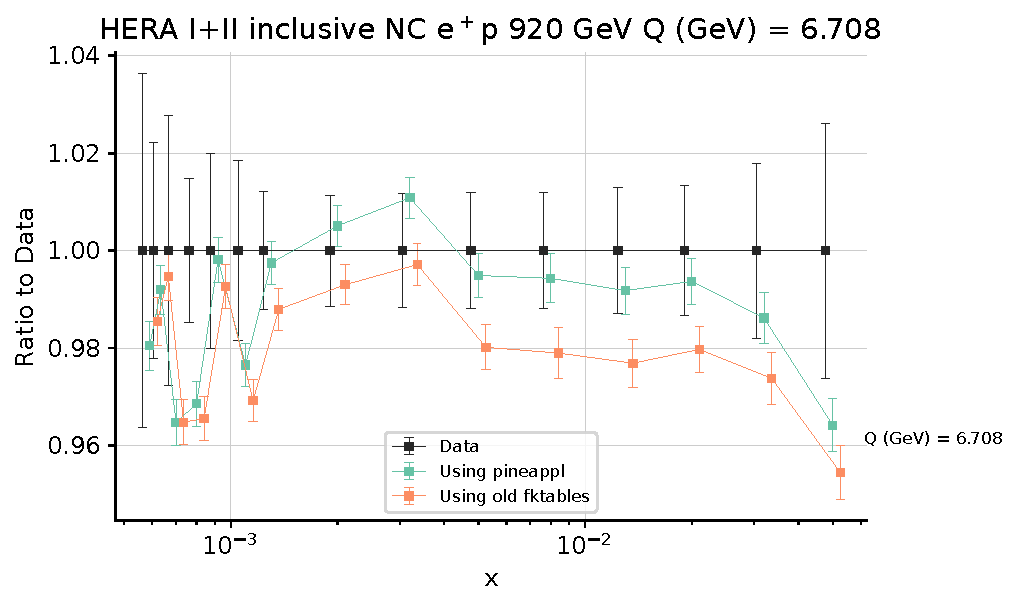
\includegraphics[width=0.48\linewidth]{
    ch-yadism/matched_datasets_from_dataspecs14_dataset_report_Datanorm_plot_fancy_dataspecs_11.pdf
  }
  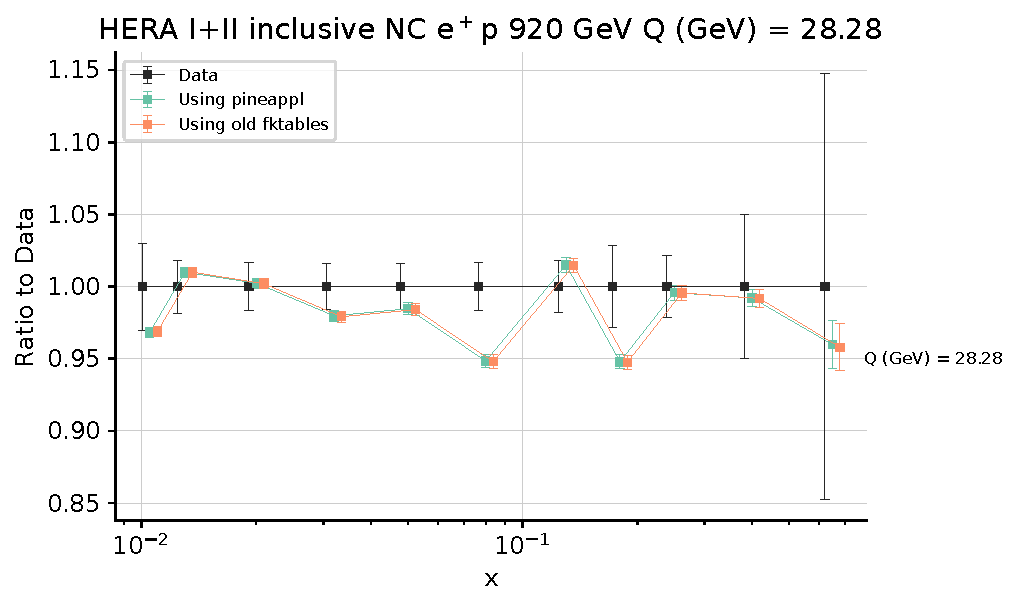
\includegraphics[width=0.48\linewidth]{
    ch-yadism/matched_datasets_from_dataspecs14_dataset_report_Datanorm_plot_fancy_dataspecs_23.pdf
  }
  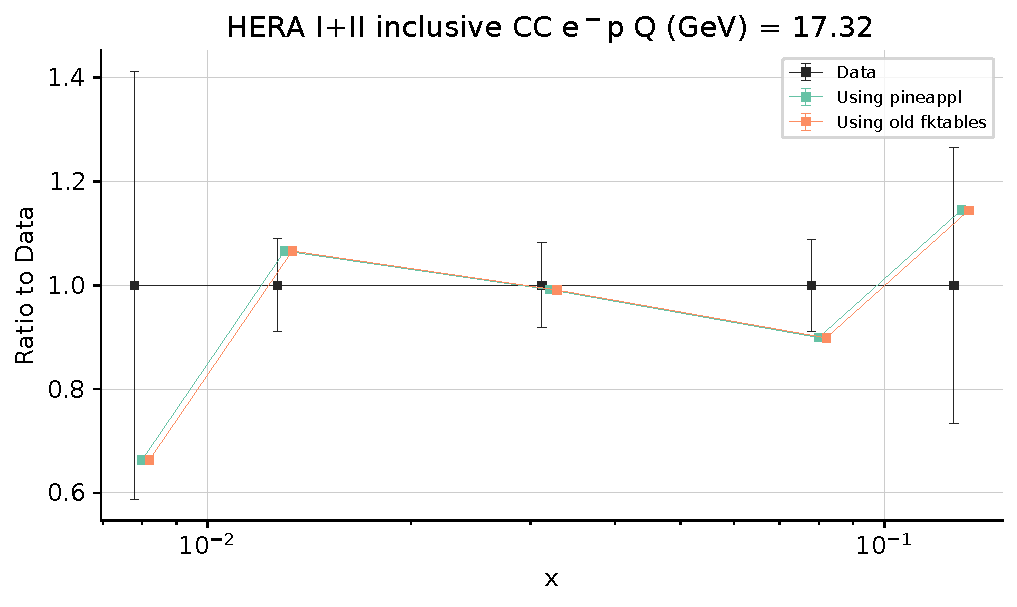
\includegraphics[width=0.48\linewidth]{
    ch-yadism/matched_datasets_from_dataspecs4_dataset_report_Datanorm_plot_fancy_dataspecs_0.pdf
  }
  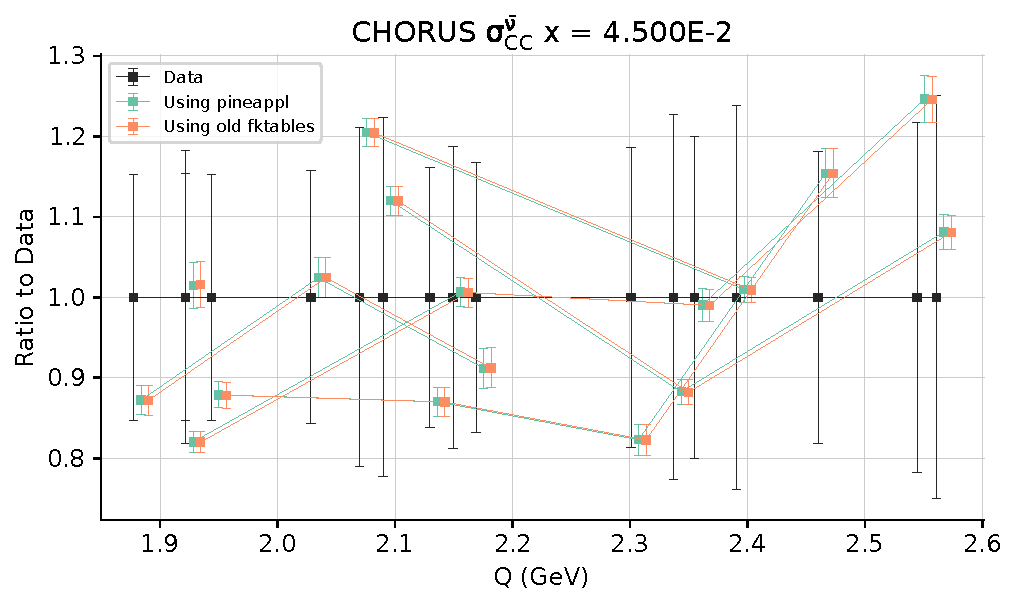
\includegraphics[width=0.48\linewidth]{
    ch-yadism/matched_datasets_from_dataspecs2_dataset_report_Datanorm_plot_fancy_dataspecs_0.pdf
  }
  \caption{
    Comparison of the \yadism predictions for DIS structure
    functions and reduced cross-sections at NNLO with the corresponding ones
    from \apfel for the same choice of input settings.
    %
    We display  predictions for four $x$ bins of representative DIS datasets
    included in the NNPDF4.0 global analysis: fixed-target neutral-current DIS
    on a deuteron target from BCDMS, fixed-target charged-current DIS on a lead
    target from CHORUS, collider neutral-current positron-proton DIS from HERA,
    and collider charged-current electron-proton DIS from HERA.
  }    
  \label{fig:dis/benchmark-apfel-yadism}
\end{figure}
%%%%%%%%%%%%%%%%%%%%%%%%%%%%%%%%%%%%%%%%%%%%%%%%%%%%%%%%%%%%%%%%%%%%%%%%%%%%%%%%%%%%%%
